\chapter{Desenvolvimento}
\label{cap:desenvolvimento}

Nesta seção, detalha-se o processo de desenvolvimento do projeto, abrangendo todas as etapas desde a concepção inicial até a implementação final utilizando os ciclos de desenvolvimento da metodologia DSR descritas na Seção \ref{sec: Fase 3 design e desenvolvimento} do capítulo de Metodologia. São apresentados os métodos, ferramentas e tecnologias utilizadas, além dos desafios enfrentados e as soluções adotadas.


\section{Ciclo 1: Fotogrametria e Construção do Modelo 3D}
\label{sec:ciclo1_fotogrametria}

\textbf{Objetivo do ciclo}: Criar um modelo 3D detalhado baseado em imagens capturadas em campo. Atender ao RFA001 (Modelo 3D de Alta Qualidade) e garantir compatibilidade com Unreal Engine 5.4. 

A seguir o processo é descrito detalhadamente.
    \subsection{Visitas de campo e Captura de Imagens} 
    Ao todo foram realizadas 3 visitas ao local de estudo, a Lapa da Pedra. 
    As primeiras visitas de campo, guiadas pelo Guia Ambiental e Condutor Cultural Noel José dos Santos, foram para estudo e planejamento da captura das imagens. O objetivo era analisar o terreno, identificar os pontos de interesse (pictoglifos e estrutura da gruta), e definir a melhor estratégia para a captura das imagens.

    Com a localização definida, e com a colaboração do professor Dr. Leomar Rufino Alves Júnior, especialista em fotogrametria, topografia, geodésia e sensoriamento remoto, deu-se início à etapa de aquisição de dados. Um veículo aéreo não tripulado (VANT) modelo Phantom 4 Standard (Figura \ref{fig:phantom 4}), equipado com câmera de alta resolução, foi utilizado para capturar imagens aéreas (Figuras \ref{fig:drone voando} e \ref{fig:drone dentro da caverna}) com superposição de pelo menos 70\% (Figura \ref{fig:fotos tiradas}, garantindo a cobertura completa da área e a precisão do modelo 3D. Simultaneamente, imagens terrestres foram coletadas com câmeras de celular e câmera fotográfica DSLR semi-profissional modelo Lumix Fz80 Panasoni, focando em detalhes específicos dos pictoglifos e da estrutura da gruta, principalmente os que estavam no teto - àrea que o drone não conseguia pegar com detalhes.

\begin{figure}[H]
    \centering
    \begin{minipage}{0.45\textwidth} 
        \centering
    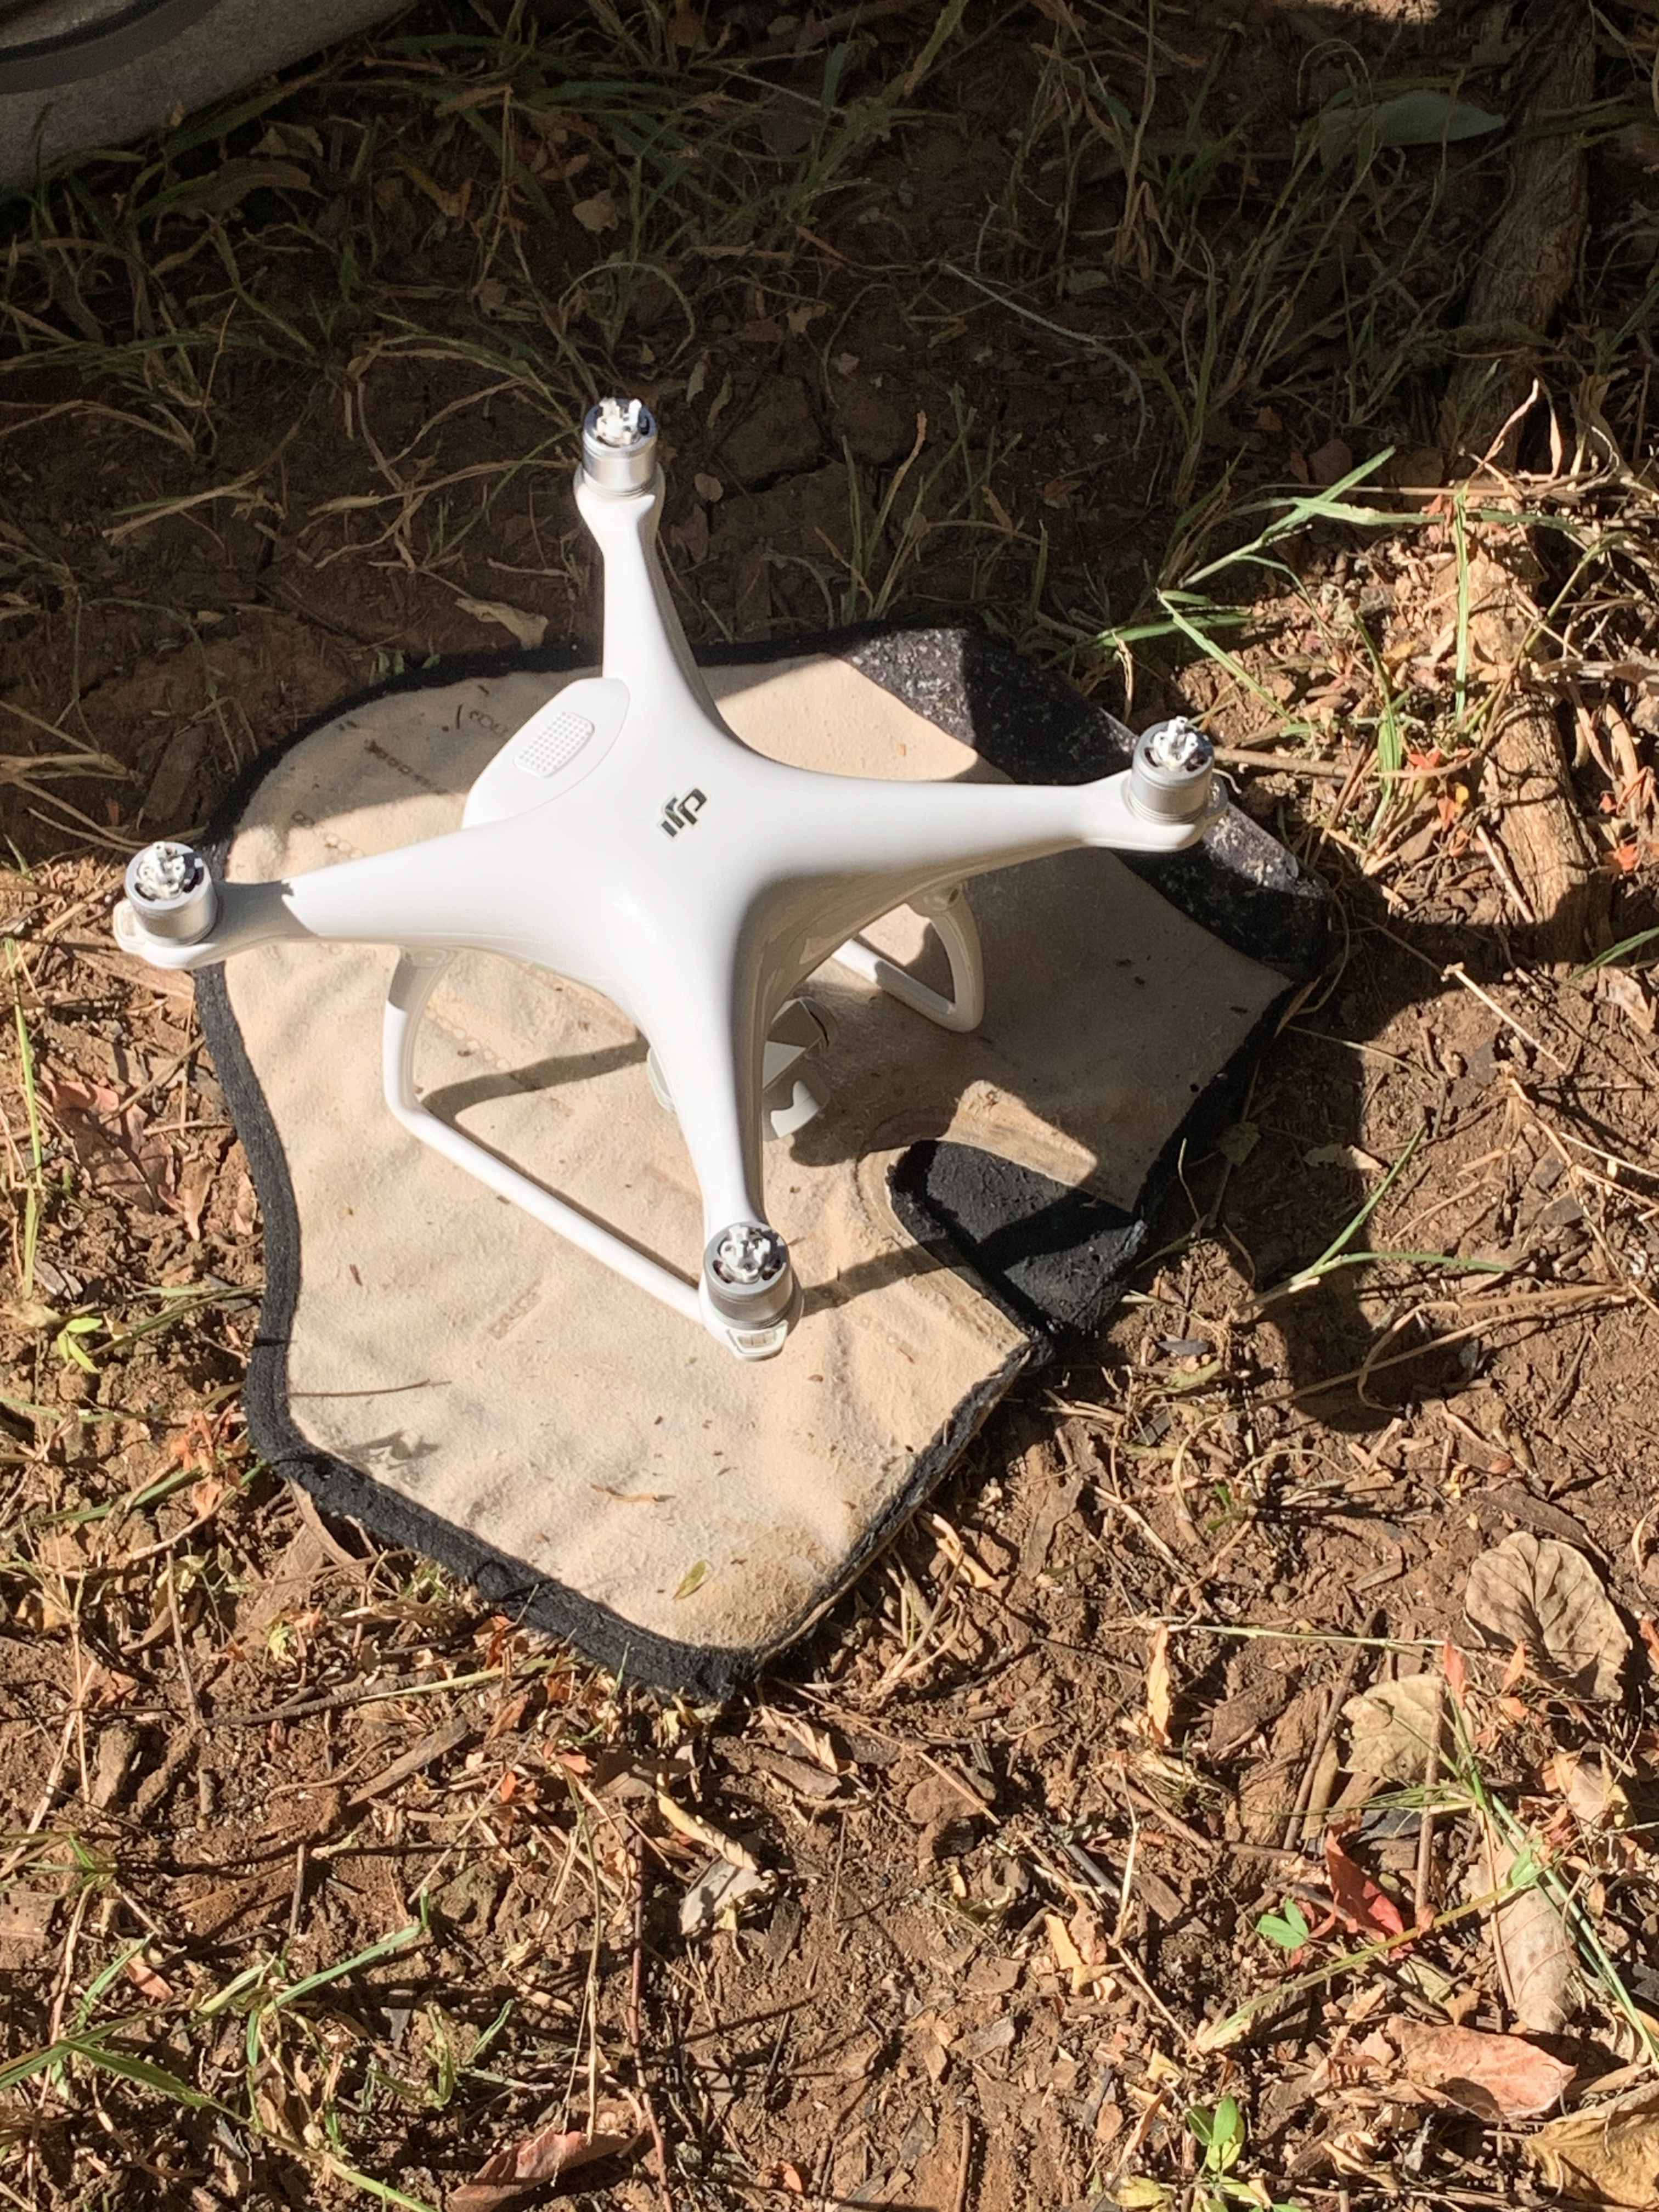
\includegraphics[height=8cm, keepaspectratio]{img/Visitas tecnicas/phantom 4.png}
    \caption{ Drone modelo Phantom 4, utilizado \\ para as capturas das imagens.\\
        \textbf{Fonte:} Acervo pessoal do Ramon Almeida.}
    \label{fig:phantom 4}   
    \end{minipage}
    \hspace{1cm} 
    \begin{minipage}{0.45\textwidth}
        \centering
        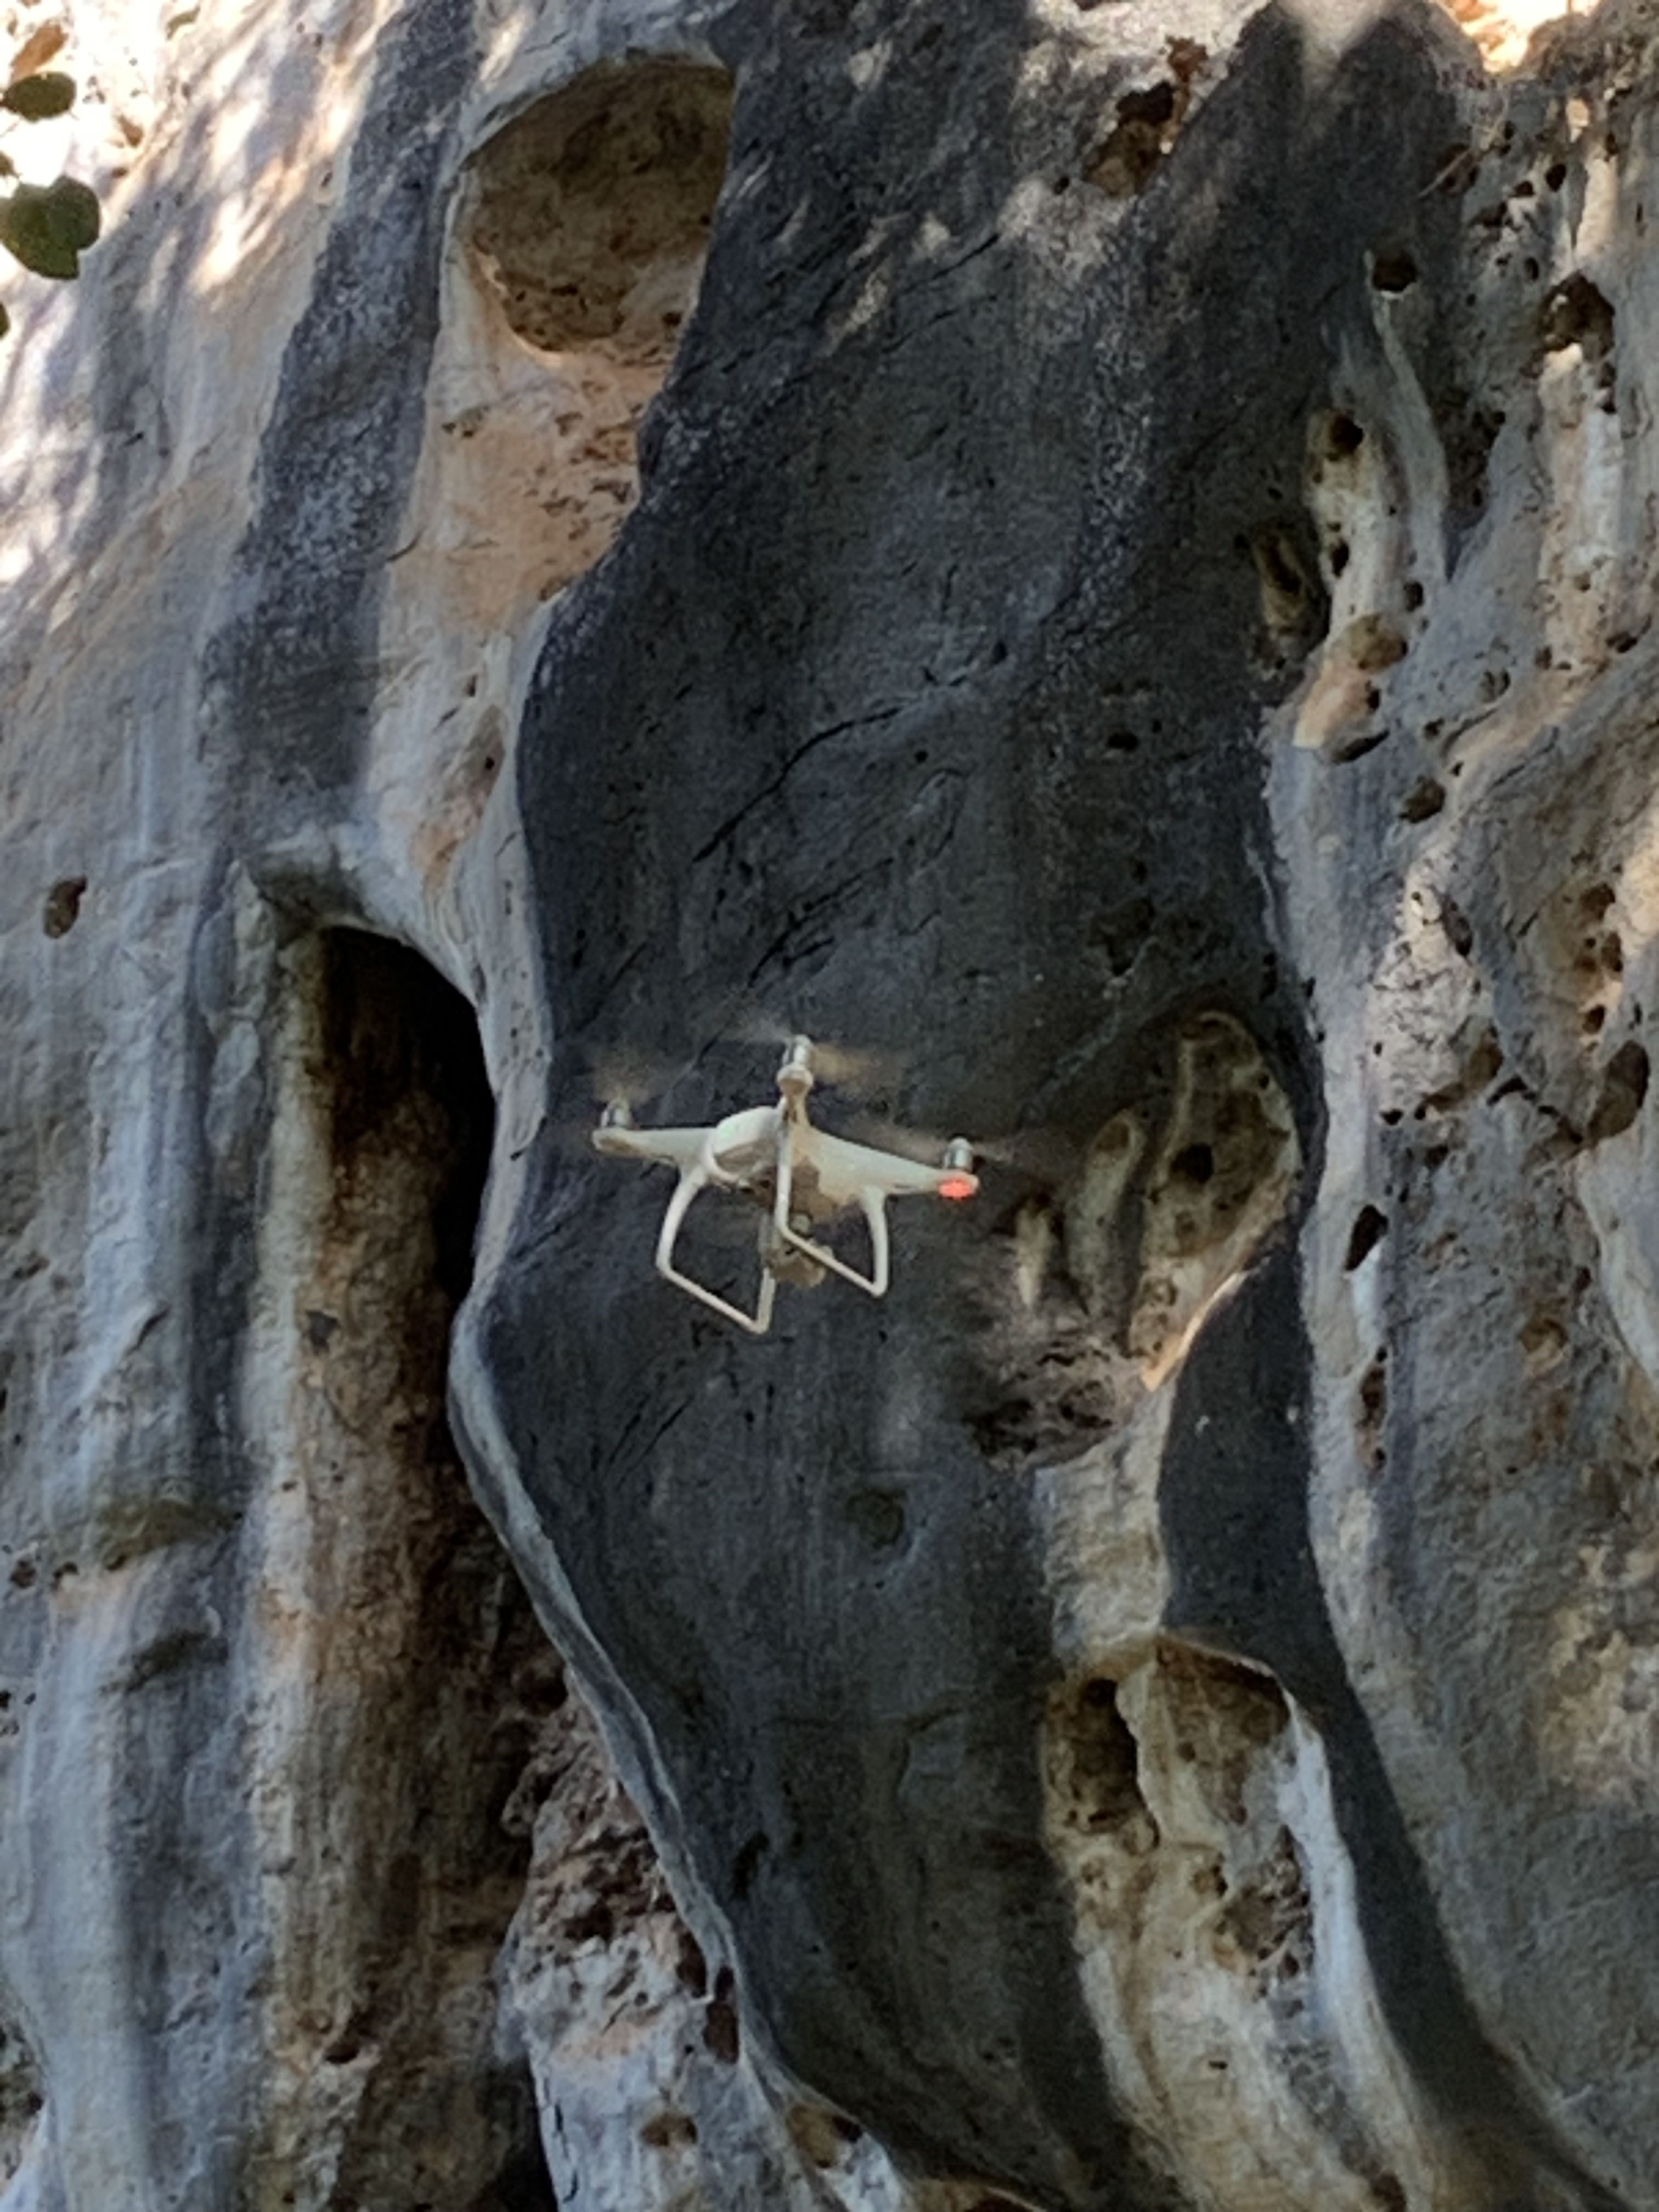
\includegraphics[height=8cm, keepaspectratio]{img/Visitas tecnicas/drone voando.png}
        \caption{Processo de captura de imagens com o \\ drone no exterior da caverna.\\
            \textbf{Fonte:} Acervo pessoal do professor Edson Borges.}
        \label{fig:drone voando}
    \end{minipage}
\end{figure}

\begin{figure}[H]
    \centering
        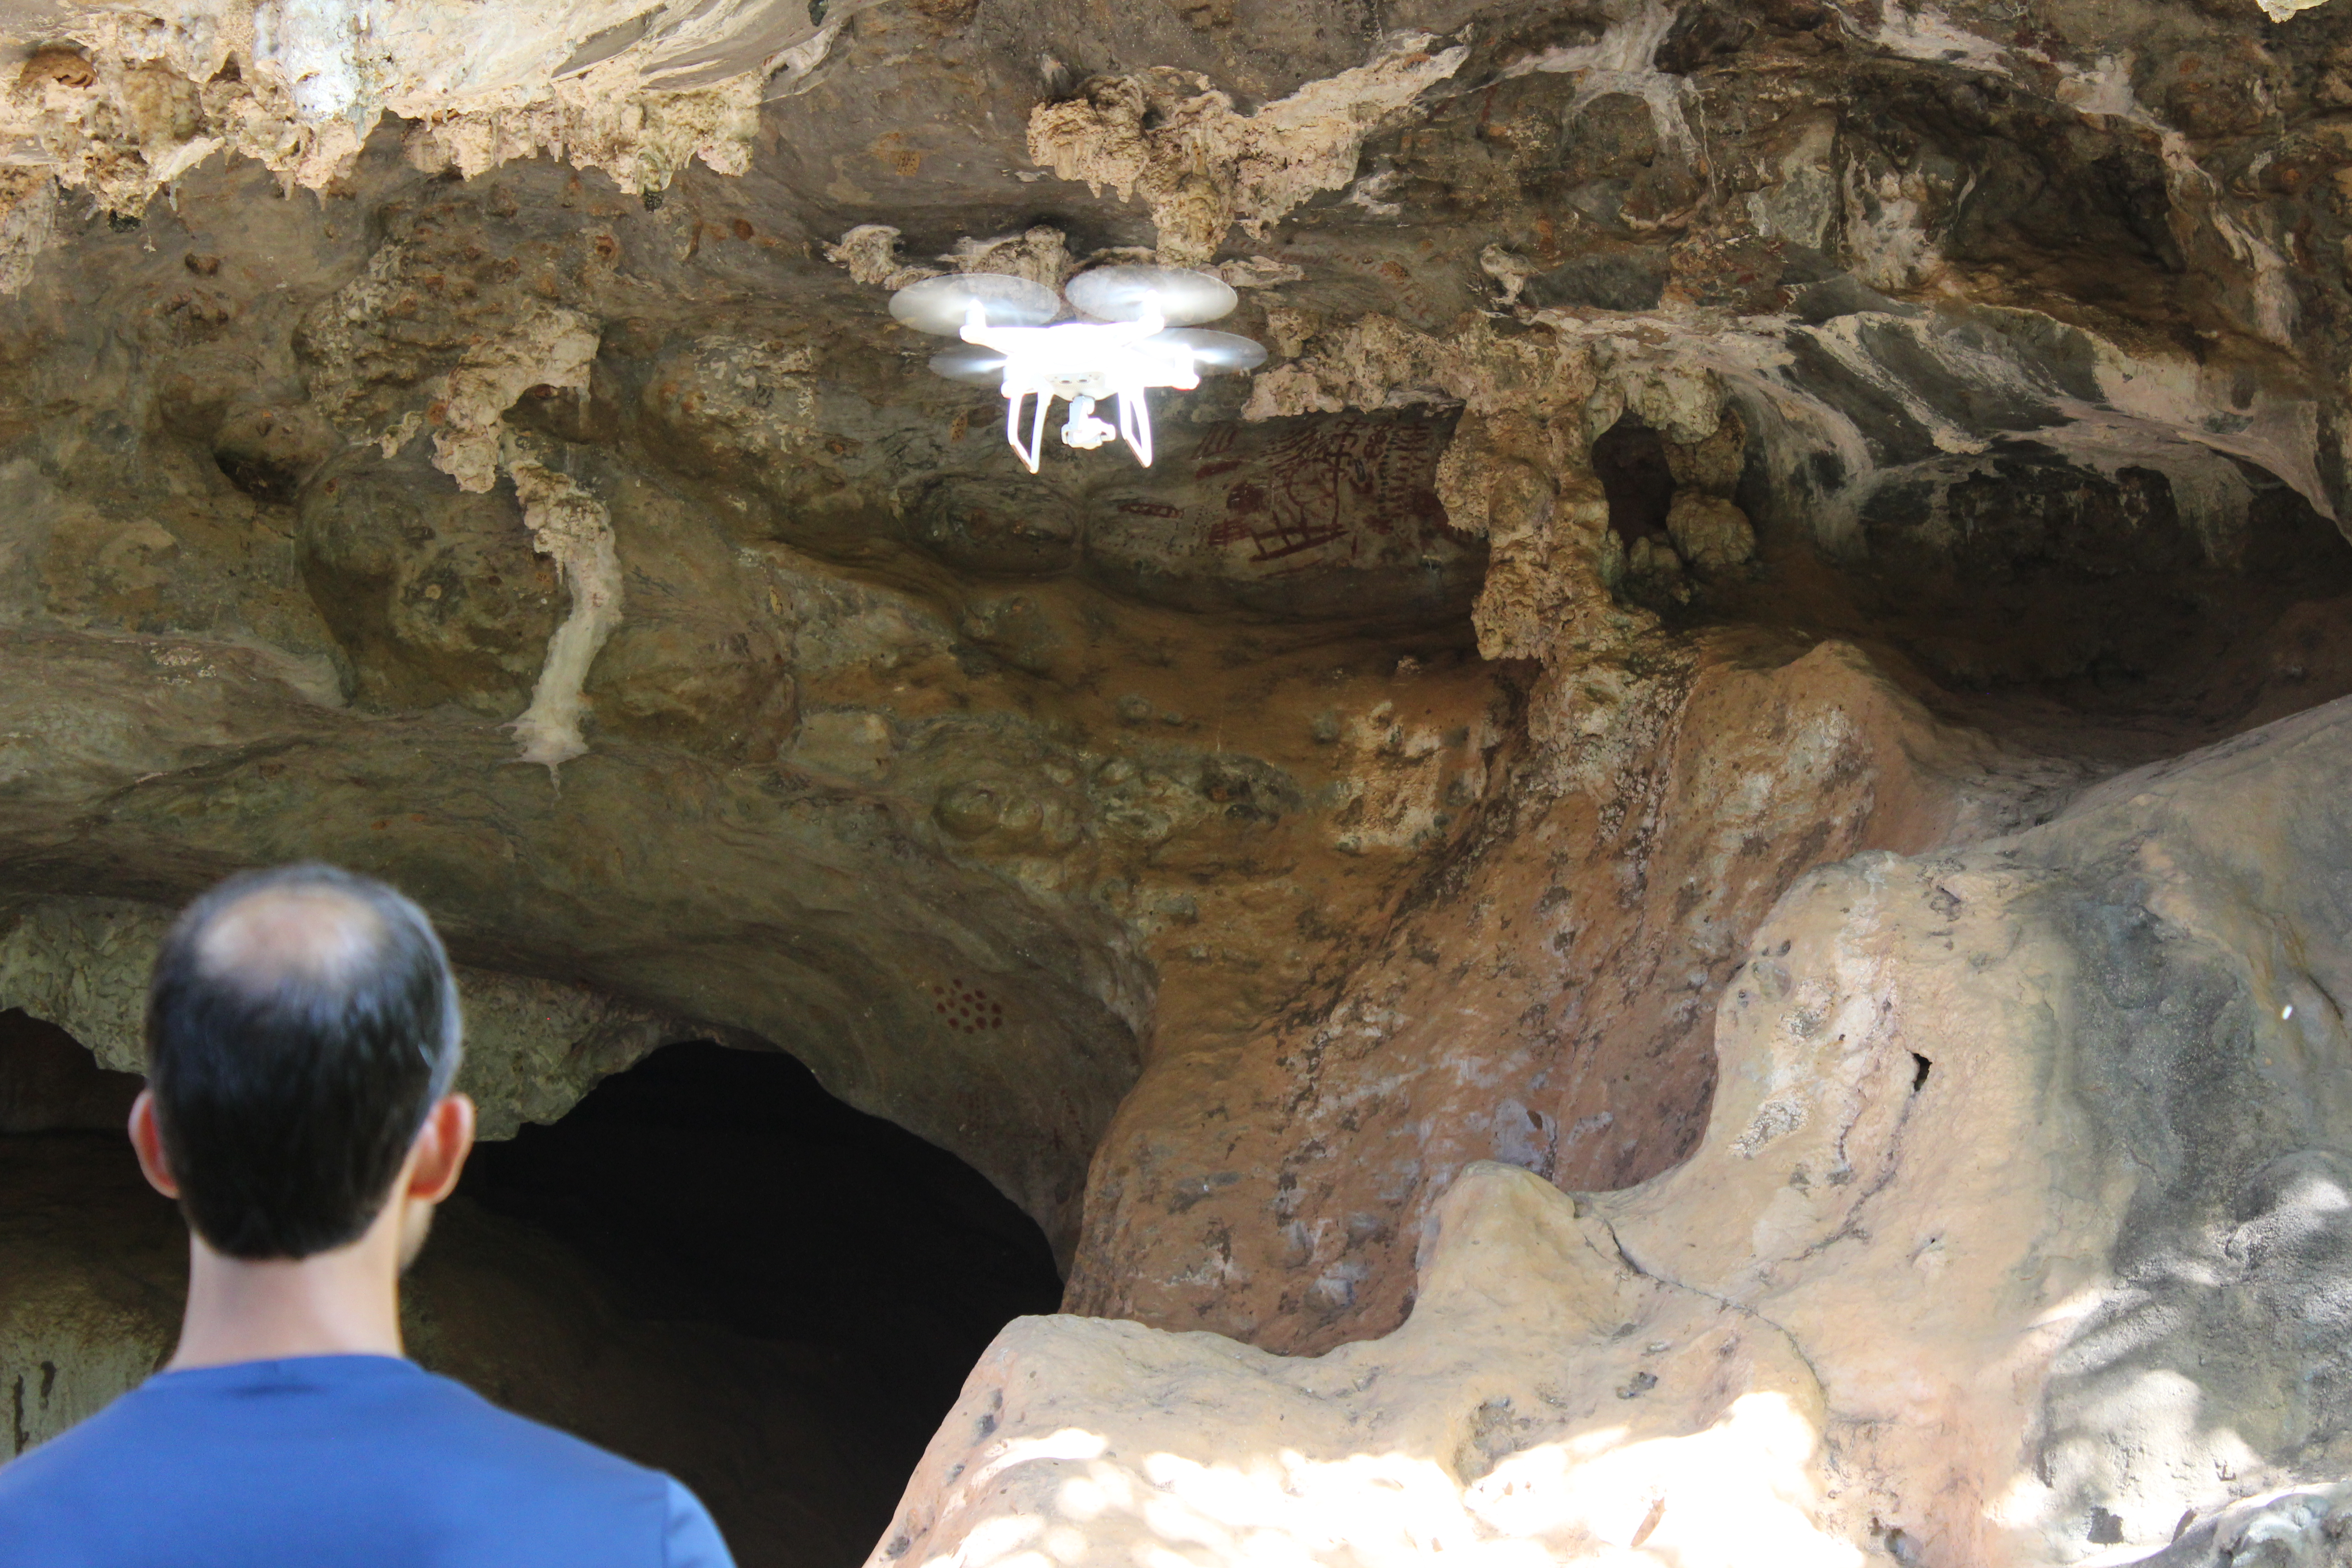
\includegraphics[height=8cm, keepaspectratio]{img/Visitas tecnicas/drone dentro da caverna.jpg}
        \caption{Processo de captura de imagens com o drone \\
        no interior da caverna. \\
            \textbf{Fonte:} Acervo pessoal do Ramon Almeida.}
        \label{fig:drone dentro da caverna}
\end{figure}

 Ao todo foram capturadas 1.493 imagens cobrindo diferentes ângulos do sítio arqueológico. Dessas fotos, 1018 foram selecionadas e as outras foram removidas por conter ruídos, desfoque ou má qualidade que poderiam atrapalhar o processo seguinte (Figura \ref{fig:fotos tiradas}).

\begin{figure}[H]
    \centering
    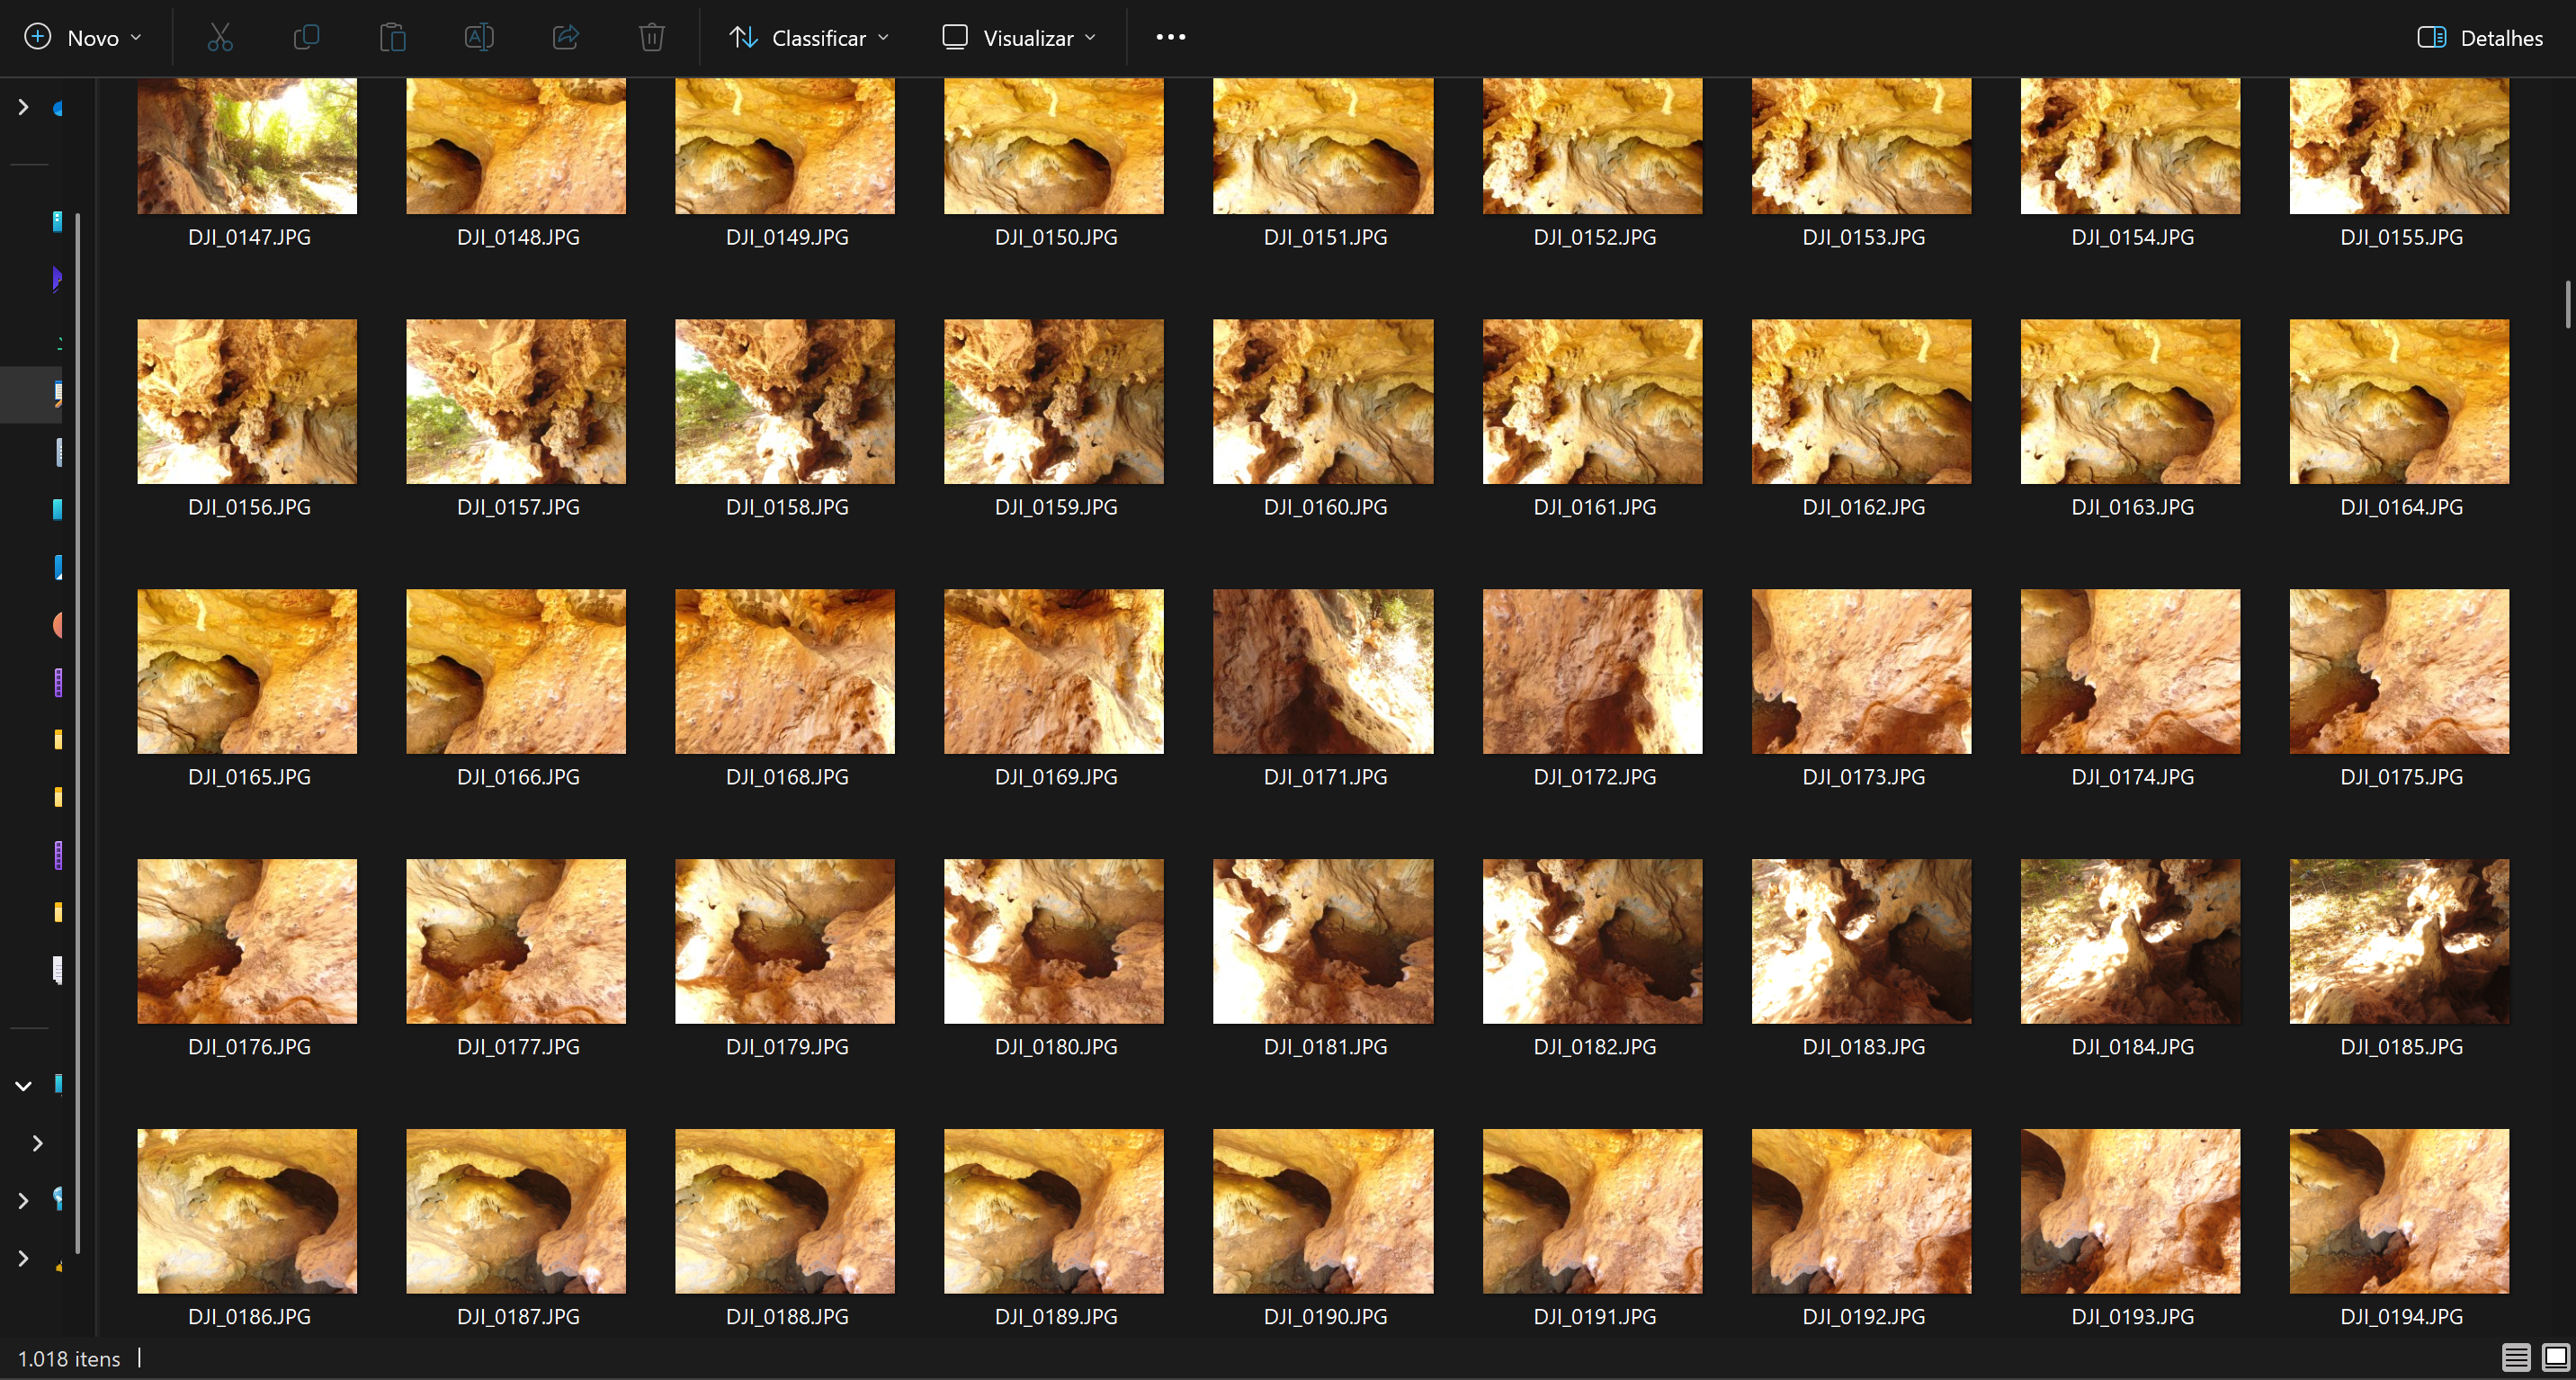
\includegraphics[height=8cm, keepaspectratio]{img/reality e fotogrametria processo/imagens capturas.png}
    \caption{Fotografias capturadas com superposição de 70\%.\\
        \textbf{Fonte:} Elaborado pelo autor, 2025.}
    \label{fig:fotos tiradas}   
\end{figure}

    \subsection{Processamento no Reality Capture para reconstrução fotogramétrica}
    \begin{enumerate}
\item \textbf{Alinhamento das Fotos} \\
Com as fotos devidamente selecionadas pôde-se seguir para a etapa de alinhamento, que ocorre no software Reality Capture. O software identifica pontos correspondentes nas imagens e calcula suas posições espaciais relativas (Figura \ref{fig:alinhamento}). Este processo resulta na criação de uma nuvem de pontos esparsa, que representa os principais elementos da cena. 
A partir da nuvem de pontos esparsa, o software gera uma nuvem de pontos densa (Figura \ref{fig:nuvem de pontos}), que contém uma quantidade significativamente maior de pontos e oferece maior detalhamento. Esta etapa é computacionalmente intensiva e depende da qualidade das imagens de entrada.

\begin{figure}[H]
    \centering
        \centering
        \includegraphics[height=8cm, keepaspectratio]{img/reality e fotogrametria processo/cameras alinhamento.png}
        \caption{Alinhamento das imagens pelo software Reality Capture. \\
            \textbf{Fonte:} Elaborado pelo autor, 2025.}
        \label{fig:alinhamento}
\end{figure}

\begin{figure}[H]
        \centering
        \includegraphics[height=8cm, keepaspectratio]{img/reality e fotogrametria processo/primeiro modelo componente.png}
        \caption{Nuvem de pontos densa. \\
            \textbf{Fonte:} Elaborado pelo autor, 2025.}
        \label{fig:nuvem de pontos}
\end{figure}


\item \textbf{Filtragem e Recorte} \\
Para eliminar pontos indesejados, como vegetação ou objetos móveis, foi realizada uma filtragem manual iterativa. Esta etapa é essencial para garantir que apenas os elementos relevantes sejam incluídos no modelo final.
\begin{figure}[H]
        \centering
        \includegraphics[height=8cm, keepaspectratio]{img/reality e fotogrametria processo/Criação de nuvem de pontos.png}
        \caption{Identificação dos pontos indesejados para filtragem. \\
            \textbf{Fonte:} Elaborado pelo autor, 2025.}
        \label{fig:filtragem}
\end{figure}

\item \textbf{Criação do Modelo 3D} \\
Com base na nuvem de pontos densa filtrada, o software gerou a malha poligonal do modelo 3D, como mostra a Figura \ref{fig:modelo 3D solido}. O modelo inicial continha 102 milhões de polígonos, resultando em um nível de detalhe extremamente alto, mas também em um arquivo muito pesado.
\begin{figure}[H]
        \centering
        \includegraphics[height=8cm, keepaspectratio]{img/reality e fotogrametria processo/modelo solido e foto.png}
        \caption{Identificação dos pontos indesejados para filtragem. \\
            \textbf{Fonte:} Elaborado pelo autor, 2025.}
        \label{fig:modelo 3D solido}
\end{figure}

\item \textbf{Texturização} \\
O processo de texturização atribuiu cores e detalhes visuais à malha poligonal, utilizando informações das imagens originais. A textura gerada foi de alta qualidade, refletindo fielmente as características do ambiente capturado (Figura \ref{fig:texturizado}). Com esse modelo as figuras pré-históricas no interior da gruta ficaram nítidas e altamente visíveis, como mostra a Figura \ref{fig:interior}.

\begin{figure}[H]
        \centering
        \includegraphics[height=8cm, keepaspectratio]{img/reality e fotogrametria processo/102M textura.png}
        \caption{Modelo texturizado de alta qualidade com 102 milhões de polígonos, parte exterior. \\
            \textbf{Fonte:} Elaborado pelo autor, 2025.}
        \label{fig:texturizado}
\end{figure}
\begin{figure}[H]
        \centering
        \includegraphics[height=8cm, keepaspectratio]{img/reality e fotogrametria processo/interior.png}
        \caption{Modelo texturizado de alta qualidade com 102 milhões de polígonos, parte interior. \\
            \textbf{Fonte:} Elaborado pelo autor, 2025.}
        \label{fig:interior}
\end{figure}
\end{enumerate}
    \subsection{Simplificação do Modelo 3D, garantindo compatibilidade com a Unreal Engine (RFA001).}
  
Devido ao tamanho do modelo inicial (102 milhões de polígonos), foi necessário realizar um processo de simplificação para torná-lo mais leve e compatível para uso em softwares como a Unreal Engine, que suporta bem até 5 milhões de polígonos. A malha foi reduzida consideravelmente tornando-o mais leve, porém a qualidade ficou muito ruim deixando os desenhos praticamente apagados, como mostra a Figura \ref{fig:modelo ruim}

\begin{figure}[H]
    \centering
    % Primeira figura
    \begin{minipage}{0.45\textwidth} % Reduzi a largura para 45%
        \centering
        \includegraphics[height=5cm, keepaspectratio]{img/reality e fotogrametria processo/modelo ruim.png}
        \caption{Modelo simplificado com 5 milhões \\ de polígonos. Desenho apagado. \\
            \textbf{Fonte:} Elaborado pelo autor, 2025.}
        \label{fig:modelo ruim}
    \end{minipage}
    \hspace{1cm} % Espaço fixo de 0.5cm entre as figuras
    % Segunda figura
    \begin{minipage}{0.45\textwidth} % Reduzi a largura para 45%
        \centering
        \includegraphics[height=5cm, keepaspectratio]{img/reality e fotogrametria processo/desenho bom retroprojeção.png}
        \caption{Modelo simplificado com reprojeção \\ de textura. \\
            \textbf{Fonte:} Elaborado pelo autor, 2025.}
        \label{fig:desenho bom}
    \end{minipage}
\end{figure}

  \subsection{Reprojeção de textura do modelo de alta resolução para o modelo simplificado, mantendo a qualidade visual.} 
  
Para manter a qualidade visual do modelo simplificado, foi aplicada a técnica de reprojeção de textura \ref{fig:desenho bom}. Essa técnica permite utilizar a textura do modelo original de alta qualidade no modelo simplificado, resultando em um equilíbrio ideal entre detalhamento visual e peso computacional. Primeiro é feito o processo de \textit{ uv unwrap}, que pode ser traduzido como "desdobramento UV" ou "mapeamento UV" (Figura \ref{fig:unwrap}). Esta etapa minimiza distorções e sobreposições, garantindo que a textura se encaixe ao objeto 3D de forma realística, facilitando a transposição de texturas de um modelo para o outro. 
\begin{figure}[H]
        \includegraphics[height=8cm, keepaspectratio]{img/reality e fotogrametria processo/unwrap.png}
        \caption{Processo de Mapeamento UV. \\
            \textbf{Fonte:} Elaborado pelo autor, 2025.}
        \label{fig:unwrap}
\end{figure}

Todo o processo no Reality Capture é demorado e cada etapa pode consumir várias horas. Um dos processos mais rápidos foi o de reprojeção de textura que demorou cerca de apenas 2 horas utilizando um Galaxybook 4 ultra com 32 Gigas de memória RAM, placa de Vídeo NVIDIA 4070 e processador Intel(R) Core(TM) Ultra 9 185H   2.50 GHz com 22 núcleos. Na Figura \ref{fig:reprojecao tempo} pode ser vista uma captura de tela do software processando a reprojeção.
\begin{figure}[H]
        \centering
        \includegraphics[height=8cm, keepaspectratio]{img/reality e fotogrametria processo/reprojeção.png}
        \caption{Processamento da reprojeção de textura. \\
            \textbf{Fonte:} Elaborado pelo autor, 2025.}
        \label{fig:reprojecao tempo}
\end{figure}


\end{enumerate}
\subsection*{Considerações Finais do Ciclo 1}
O processo de fotogrametria no Reality Capture demonstrou ser uma ferramenta poderosa para a geração de modelos 3D detalhados. A combinação de técnicas como a simplificação de malhas e a reprojeção de textura permitiu criar modelos otimizados para uso em softwares como a Unreal Engine, mantendo alta qualidade visual. Este fluxo de trabalho é essencial para aplicações em um ambiente virtual, a qual é a próxima etapa.


% Ciclo 2
\section{Ciclo 2: Construção do Ambiente Virtual na Unreal Engine}
\label{sec:ciclo2_unreal}
\label{sec:ciclo2_unreal}
A escolha da plataforma Unreal Engine 5.4 para a criação do ambiente virtual 3D se justifica pela sua capacidade de gerar experiências imersivas e interativas. O Unreal Engine é um motor de criação de jogos amplamente utilizado na indústria de jogos, cinema e arquitetura. A plataforma oferece recursos como simulação de luz, movimentações de câmera e personagens, e a possibilidade de interagir com os elementos do ambiente, tornando o ambiente virtual 3D mais realista e envolvente \citep{silva2022realidade}.

\textbf{Objetivo do ciclo}: Desenvolver um ambiente virtual interativo na Unreal Engine 5.4 que atenda aos requisitos funcionais RFA002 (Navegação em Terceira Pessoa), RFA003 (Alternância de Câmera), RFA004 (Avatar Personalizado), bem como aos requisitos não funcionais RNFA001 (Compatibilidade com Windows) e RNFA002  (Instalação Simplificada). Este ciclo aborda a importação do modelo 3D otimizado, a criação do cenário virtual, a implementação de funcionalidades interativas e a preparação para distribuição.

\subsection{Importação do Modelo 3D Otimizado na Unreal Engine 5.4}
O modelo 3D simplificado e texturizado, gerado no Reality Capture durante o Ciclo 1, foi importado para a Unreal Engine 5.4. Durante a importação, foram realizados ajustes nas propriedades do modelo, incluindo:
\begin{enumerate}
    \item \textbf{Escala e Posicionamento}: O modelo foi ajustado para corresponder à escala do ambiente virtual, garantindo que as proporções fossem consistentes com os outros elementos do cenário. A Figura \ref{fig:escala} mostra uma foto real de um ser humano como referência de tamanho para o ajuste de proporção do modelo 3D.
    \item \textbf{Otimização de Materiais}: Os materiais do modelo foram ajustados para aproveitar o sistema Nanite da Unreal Engine, que permite renderizar geometrias complexas sem comprometer o desempenho.
    \item \textbf{Colisão}: Foram configuradas colisões automáticas para permitir interações realistas entre o avatar e o ambiente. Em áreas específicas, como entradas e interior da gruta, foram criadas colisões personalizadas para garantir precisão. Como mostrado na Figura \ref{fig:colisao}
\end{enumerate}
% A Figura \ref{fig:modelo_importado} ilustra o modelo 3D após a importação e ajustes iniciais.

\begin{figure}[H]
        \centering
        \includegraphics[height=6cm, keepaspectratio]{img/unreal/escala.png}
        \caption{Ajuste na escala comparando com uma foto real de\\ um ser humano na entrada da gruta. \\
            \textbf{Fonte:} Elaborado pelo autor, 2025.}
        \label{fig:escala}
\end{figure}

\begin{figure}[H]
        \centering
        \includegraphics[height=8cm, keepaspectratio]{img/unreal/colisão.png}
        \caption{Colisão dos objetos na cena dentro da Unreal Engine. \\
            \textbf{Fonte:} Elaborado pelo autor, 2025.}
        \label{fig:colisao}
\end{figure}


\subsection{Criação do Cenário Virtual}
Para enriquecer o ambiente virtual, foram adicionados elementos complementares ao modelo principal, como vegetação, gramado, pedras e um terreno detalhado. Esses elementos foram criados utilizando \textit{assets} disponíveis no \textit{Marketplace} da \textit{Unreal Engine} e customizados para se integrar harmoniosamente ao modelo 3D da Lapa da Pedra. As principais etapas incluem:
\begin{enumerate}
    \item \textbf{Texturas Realistas}: Foram aplicadas texturas de alta qualidade para criar uma aparência naturalista. A iluminação dinâmica foi configurada para interagir realisticamente com as superfícies, destacando detalhes como sombras e reflexos.
    \item \textbf{Iluminação Dinâmica}: Utilizando o sistema Lumen da Unreal Engine, foi implementada uma iluminação global dinâmica, que simula a interação de luz natural com o ambiente. Isso incluiu a configuração de fontes de luz direcionais para simular o sol e luzes pontuais para áreas internas da gruta.
    \item \textbf{Ambientação Sonora}: Sons ambientes, como vento e pássaros, foram adicionados para aumentar a imersão do usuário no cenário virtual.
\end{enumerate}
A Figura \ref{fig:grama} apresenta o cenário virtual sendo preenchido com elementos de paisagem como árvores, rochas, grama com o modelo 3D integrado ao ambiente.
\begin{figure}[H]
        \centering
        \includegraphics[height=8cm, keepaspectratio]{img/unreal/paisagem grass.png}
        \caption{Processo de criação e preenchimento do cenário. \\
            \textbf{Fonte:} Elaborado pelo autor, 2025.}
        \label{fig:grama}
\end{figure}


\subsection{Implementação do Sistema de Navegação em Terceira Pessoa (RFA002)}
Foi desenvolvido um sistema de navegação em terceira pessoa, permitindo que o usuário controle um avatar interativo e explore o ambiente virtual. Para isso, foi utilizado o Template de Terceira Pessoa fornecido pela Unreal Engine, que foi adaptado para atender às necessidades específicas do projeto. As principais funcionalidades incluem:
\begin{itemize}
    \item Movimentação suave do avatar com controles de teclado e mouse.
    \item Detecção de colisão para evitar que o avatar atravesse paredes ou obstáculos.
\end{itemize}

\subsection{Criação de Avatar Personalizado no Metahuman (RFA004)}
Um avatar personalizado foi criado utilizando o Metahuman Creator, uma ferramenta da Unreal Engine para geração de personagens humanos altamente realistas. O avatar foi projetado para se assemelhar ao professor Edson Borges, com base em referências fotográficas fornecidas. As etapas incluíram a modelagem facial detalhada no Metahuman Creator; a customização barba, roupas e acessórios para refletir a aparência do professor e a importação do avatar para a Unreal Engine e integração com o sistema de controle de personagem (Figura \ref{fig:metahumancamera}).
\end{enumerate}

A Figura \ref{fig:metahumanEdsonn} exibe o avatar finalizado no ambiente virtual.

\begin{figure}[H]
        \centering
\includegraphics[height=8cm, keepaspectratio]{img/unreal/ajuste de câmera edson.png}
        \caption{Importação do Metahuman do professor Edson \\ para se tornar um personagem controlável. \\
            \textbf{Fonte:} Elaborado pelo autor, 2025.}
        \label{fig:metahumancamera}
\end{figure}

\begin{figure}[H]
        \centering
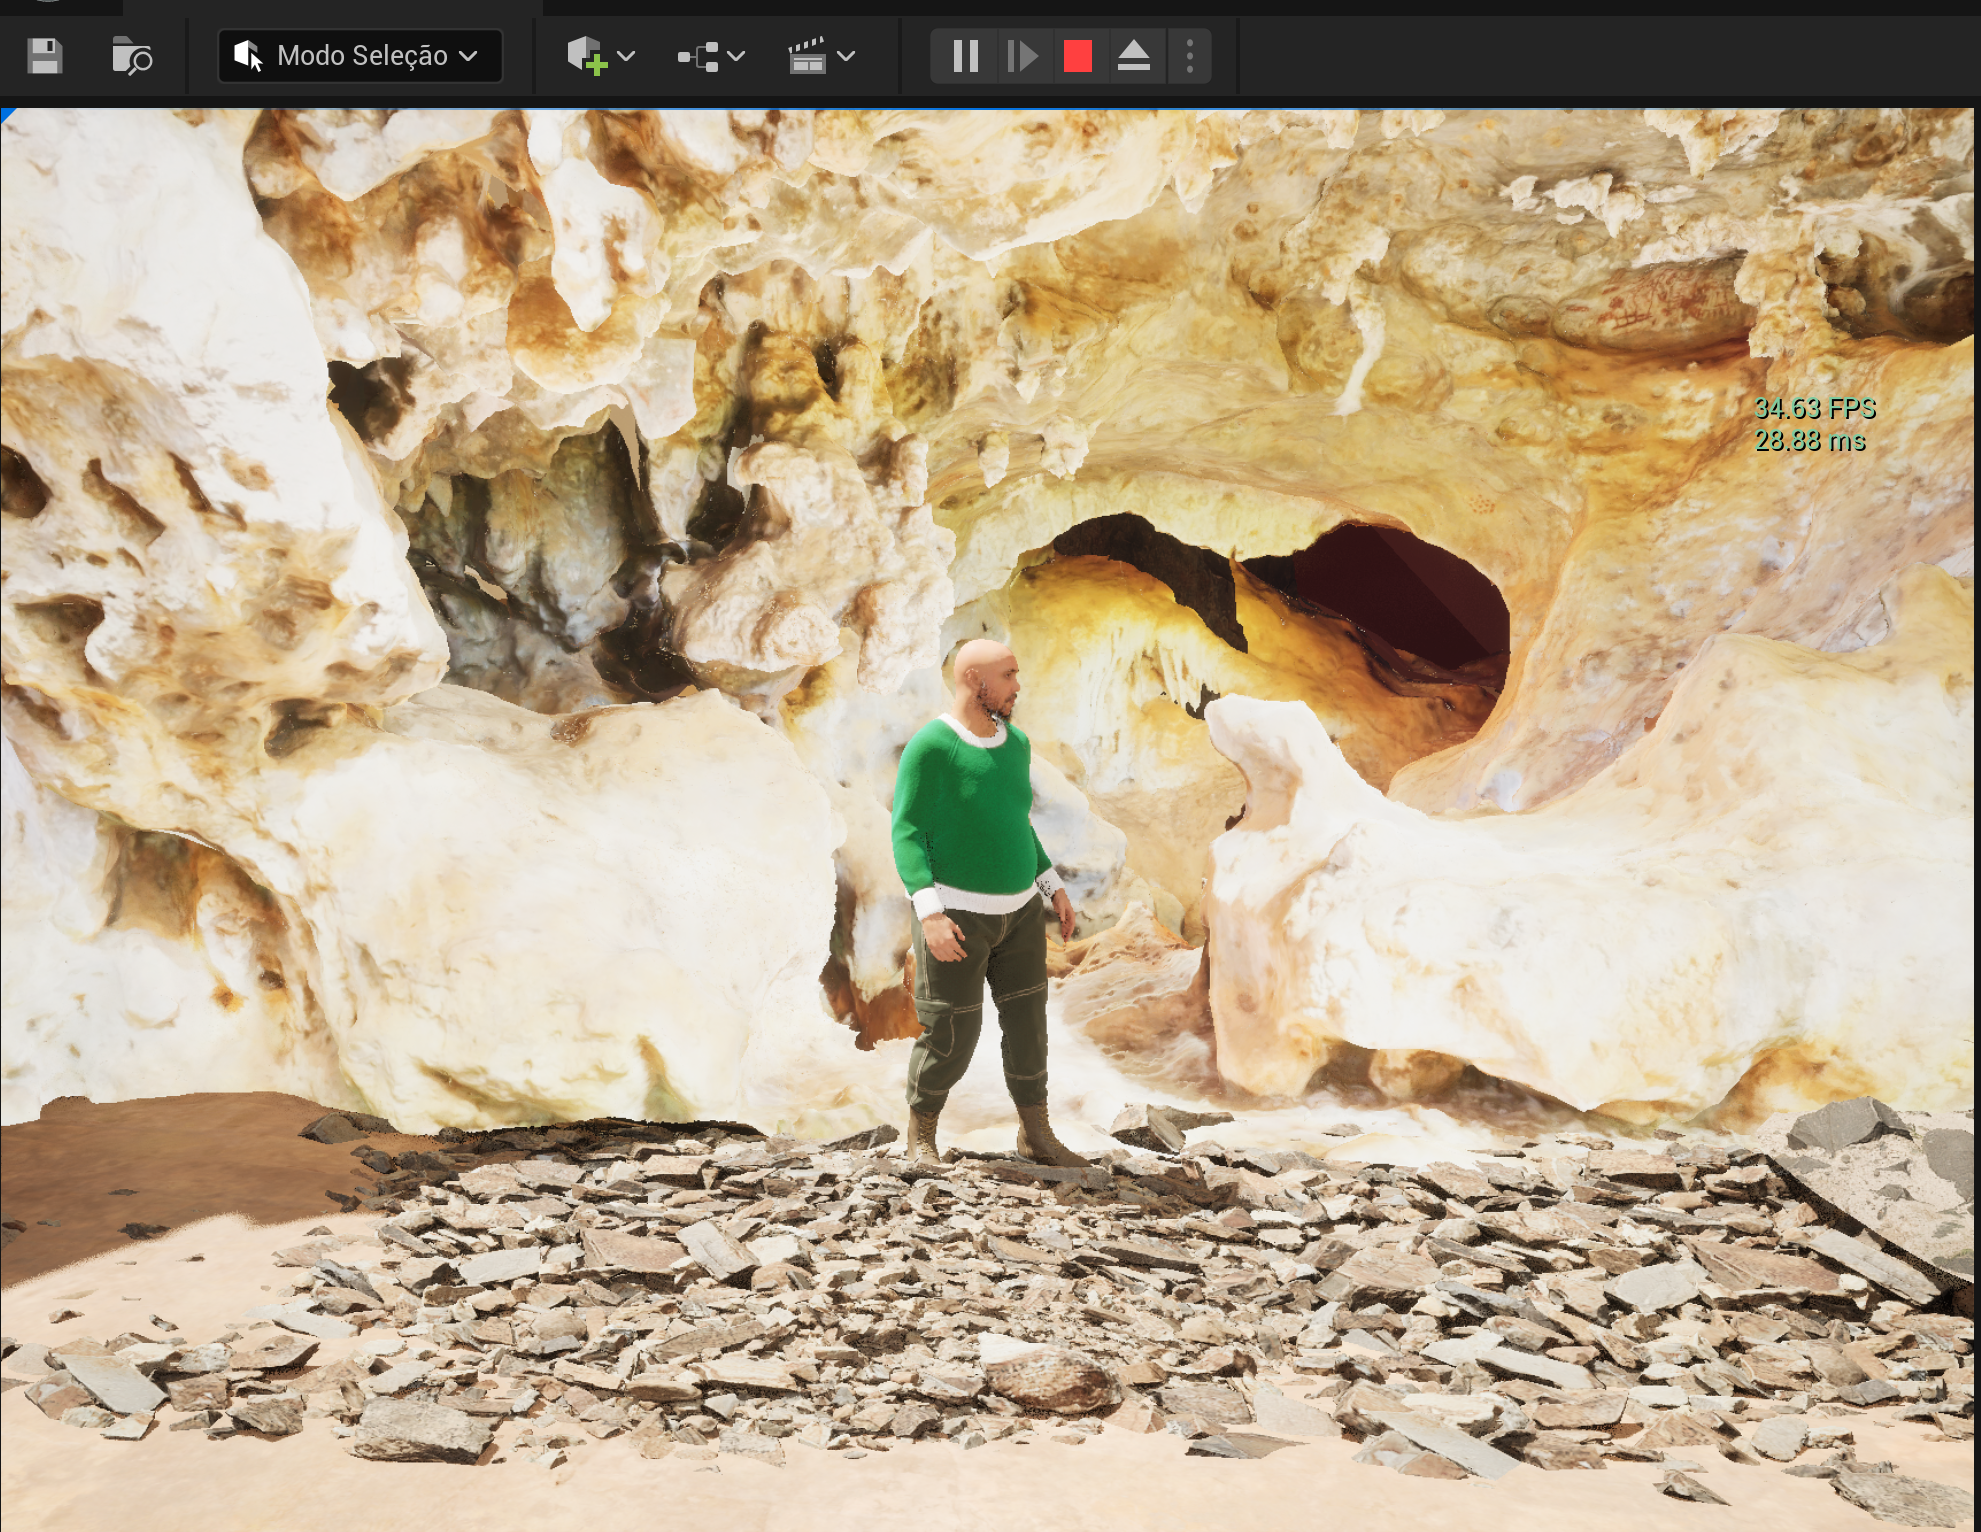
\includegraphics[height=8cm, keepaspectratio]{img/unreal/metahuman dentro da caverna.png}
        \caption{Avatar digital do professor Edson Borges no ambiente virtual. \\
            \textbf{Fonte:} Elaborado pelo autor, 2025.}
        \label{fig:metahumanEdsonn}
\end{figure}


\subsection{Desenvolvimento do Sistema de Alternância de Câmera (RFA003)}
Foi implementado um sistema de alternância de câmera, permitindo que o usuário alterne entre visão em primeira e terceira pessoa. Essa funcionalidade foi desenvolvida utilizando \textit{Blueprints}\footnote{\href{https://dev.epicgames.com/community/learning/tutorials/K8Gx/unreal-engine-comparacao-entre-blueprints-e-c-casos-de-uso}{\textit{Blueprint}} é a linguagem de programação baseada em nós da Unreal Engine. Depois ela é convertida na linguagem de programação C++. }, a linguagem visual de programação da Unreal Engine. O sistema inclui ajustes na posição e orientação das câmeras para garantir uma experiência imersiva e um botão dedicado para alternar entre as câmeras.

A Figura \ref{fig:config_camera} mostra o processo de posicionamento e configuração da câmera. A Figura \ref{fig:alternarcamera} ilustra a alternância de câmera em funcionamento.
Foi configurada a tecla "C"  como sendo responsável por alternar entre as câmeras, e a configuração da \textit{Blueprint} utilizada pode ser vista na Figura \ref{fig:blueprint_camera}.

\begin{figure}[H]
        \centering
        \includegraphics[height=8cm, keepaspectratio]{img/unreal/ajuste de câmera 1ºpessoa.png}
        \caption{Ajuste da câmera para visualização primeira pessoa. \\
            \textbf{Fonte:} Elaborado pelo autor, 2025.}
        \label{fig:config_camera}
\end{figure}

\begin{figure}[H]
        \centering
        \includegraphics[height=6cm, keepaspectratio]{img/unreal/1 pessoa e 3 pessoa comparacao.png}
        \caption{Ajuste de posicionamento da câmera do avatar.
            \textbf{Fonte:} Elaborado pelo autor, 2025.}
        \label{fig:alternarcamera}
\end{figure}

\begin{figure}[H]
        \centering
        \includegraphics[height=8cm, keepaspectratio]{img/unreal/blueprint troca de câmera.png}
        \caption{Lógica da \textit{Blueprint} para troca de câmeras
            \textbf{Fonte:} Elaborado pelo autor, 2025.}
        \label{fig:blueprint_camera}
\end{figure}

\subsection{Criação de Tela de Menu}
Uma tela de menu inicial foi desenvolvida para facilitar a navegação e a interação do usuário. A tela inclui opções como iniciar o ambiente virtual, visitar o site, sair do aplicativo e descrição dos controles.
A interface foi projetada para ser intuitiva e esteticamente agradável, utilizando \textit{widgets}\footnote{Widgets são elementos de interação em interfaces gráficas, como janelas, botões e menus, que facilitam o acesso a aplicativos e ferramentas.} da \textit{Unreal Engine}. A Figura \ref{fig:tela_menu} mostra a tela de menu finalizada.

\begin{figure}[H]
        \centering
        \includegraphics[height=8cm, keepaspectratio]{img/unreal/menu com controles.png}
        \caption{Tela de menu do ambiente virtual. \\
            \textbf{Fonte:} Elaborado pelo autor, 2025.}
        \label{fig:tela_menu}
\end{figure}


\subsection{Empacotamento do Ambiente Virtual e Criação de Instalador (RNFA003)}
O ambiente virtual foi empacotado em um arquivo executável (.exe) para distribuição. Para facilitar a instalação por usuários finais, foi criado um instalador utilizando o software \textit{Inno Setup}. A Figura \ref{fig:configuracao_inno_setup} representa a interface de desenvolvimento do instalador, que após configurado é compilado para ser executado em Windows.

\begin{figure}[H]
        \centering
        \includegraphics[height=8cm, keepaspectratio]{img/Inno setup/configuracao do instalador.png}
        \caption{Configurações iniciais para construir o instalador \\ na ferramenta Inno Setup \\
            \textbf{Fonte:} Elaborado pelo autor, 2025.}
        \label{fig:configuracao_inno_setup}
\end{figure}

Com o instalador criado basta dar um duplo clique no arquivo para começar o processo. O instalador inclui:
\begin{itemize}
    \item Suporte para instalação em múltiplos idiomas, demonstrado na Figura \ref{fig:idiomas};
    \begin{figure}[H]
        \centering
        \includegraphics[height=8cm, keepaspectratio]{img/Inno setup/multiidiomas.png}
        \caption{Interface do instalador do ambiente virtual personalizado pelo \textit{Inno Setup }\\ com suporte a múltiplos idiomas \\
            \textbf{Fonte:} Elaborado pelo autor, 2025.}
        \label{fig:idiomas}
\end{figure}

    \item Interface simples e intuitiva, como demonstrado no fluxo de instalação da Figura \ref{fig:fluxo};
    \begin{figure}[H]
        \centering
        \includegraphics[height=12cm, keepaspectratio]{img/Inno setup/fluxo de instalação.png}
        \caption{Fluxo de instalação após a escolha do idioma. \\
            \textbf{Fonte:} Elaborado pelo autor, 2025.}
        \label{fig:fluxo}
\end{figure}

    \item Atalhos para a Área de Trabalho e Menu Iniciar (Figura \ref{fig:atalho_icone}). 
    \begin{figure}[H]
        \centering
        \includegraphics[height=8cm, keepaspectratio]{img/Inno setup/íconearea de trabalho.png}
        \caption{Atalho para o programa gerado na área de trabalho \\
            \textbf{Fonte:} Elaborado pelo autor, 2025.}
        \label{fig:atalho_icone}
\end{figure}
    
\end{itemize}




\subsection*{Considerações Finais do Ciclo 2}
O Ciclo 2 resultou na criação de um ambiente virtual interativo e imersivo, integrando o modelo 3D otimizado da Lapa da Pedra a um cenário rico e funcional na Unreal Engine 5.4. O ambiente virtual gerado nessa etapa está pronto para ser disponibilizado para distribuição no site que será construído nas etapas posteriores.



% Ciclo 3

% \textbf{Objetivo}: Criar um protótipo de alta fidelidade para o site.

% \textbf{Processo}:
% \begin{itemize}
%     \item Criação de uma identidade visual
%     \item Definição da arquitetura da informação e wireframes.
%     \item Desenvolvimento do protótipo no Figma.
%     \item Validação do design com stakeholders.
% \end{itemize}

\section{Ciclo 3: Prototipação do Novo Site}
\label{sec:ciclo3_site}

\textbf{Objetivo do Ciclo}: Desenvolver um protótipo o novo site, atendendo aos requisitos funcionais RFS002 (Exibir Galeria de Imagens), RFS006 (Buscar Trabalhos por Filtros) e RFS007 (Informações de Contato), bem como aos requisitos não funcionais RNFS006 (Acessibilidade), RNFS008 (Responsividade) e RNFS012 (SEO).

\subsection{Análise das Referências e Inspirações}
O processo teve início com uma análise detalhada das referências e inspirações fornecidas pelo professor Edson Borges por meio de entrevista e questionário, disponível no Apêndice \ref{ap:entrevista}. Essas referências incluíam exemplos de sites educacionais, culturais e interativos, que serviram como base para alinhar as expectativas e a visão do projeto. A análise permitiu identificar elementos-chave, como estilo visual minimalista e moderno, ênfase na acessibilidade e usabilidade, e coerência com a identidade cultural de páginas de Arqueologia. A Figura \ref{fig:inpirações} ilustra algumas das referências analisadas durante esta etapa, que foram colocadas lado a lado no Figma.

\begin{figure}[H]
    \centering
    \includegraphics[height=6cm, keepaspectratio]{img/Protótipo/inspiração.png}
    \caption{ Inspirações de outros sites de Arqueologia, sites com boa estética, \\ paleta de cores ou forma atrativa. \\
        \textbf{Fonte:} Elaborado pelo autor, 2025.}
    \label{fig:inpirações}
\end{figure}

\subsection{Reorganização da Arquitetura da Informação}
Com base nas referências, foi realizada uma reorganização da arquitetura da informação do site, agrupando conteúdos relevantes, reduzindo informações desnecessárias e minimizando a quantidade de cliques necessários para que os usuários encontrassem as informações desejadas. Foi criada uma navegação hierárquica clara, com menus organizados por categorias principais, como "Página Inicial", "Sítios Arqueológicos", "Trabalhos Escritos", "Blog" e "Contato". Além disso, páginas secundárias foram eliminadas para evitar sobrecarga de conteúdo, e links rápidos foram adicionados para facilitar o acesso às principais funcionalidades do site, como o ambiente virtual e o download do instalador. Essas mudanças garantiram maior eficiência na navegação.

\subsection{Criação de Wireframes}
Para estruturar a interface do site, foram criados \textit{wireframes}\footnote{Wireframes são esboços visuais simplificados que representam a estrutura básica de uma interface, sem detalhes de design final, como cores ou imagens. Eles ajudam a planejar a disposição dos elementos na tela.} que definiram a disposição dos elementos visuais e interativos. Os \textit{wireframes} focaram em um layout responsivo, adaptável a diferentes dispositivos, como desktops, tablets e celulares, além de garantir um posicionamento estratégico de botões, menus e conteúdos prioritários. O espaçamento adequado entre os elementos foi planejado para facilitar a leitura e a interação. As Figuras \ref{fig:wireframes} e \ref{fig:wireframe} apresentam alguns dos \textit{wireframes} desenvolvidos durante esta fase.


\begin{figure}[H]
    \centering
    \begin{minipage}[b]{0.48\textwidth}
        \centering
        \includegraphics[height=8cm, keepaspectratio]{img/Protótipo/wireframes.png}
        \caption{Wireframes de baixa fidelidade \\no Figma. \\
            \textbf{Fonte:} Elaborado pelo autor, 2025.}
        \label{fig:wireframes}
    \end{minipage}
    \hfill
    \begin{minipage}[b]{0.48\textwidth}
        \centering
        \includegraphics[height=8cm, keepaspectratio]{img/Protótipo/wireframe.png}
        \caption{Wireframe de baixa fidelidade\\ no Figma ampliado. \\
            \textbf{Fonte:} Elaborado pelo autor, 2025.}
        \label{fig:wireframe}
    \end{minipage}
\end{figure}

% \subsection{Definição da Paleta de Cores e Tipografia}
% Foi definida uma paleta de cores e tipografia que refletisse a identidade visual do projeto com tons ocres, vermelhos, pretos, cinzas e brancos. Tons terrosos e verdes, inspirados nas cores das artes rupestres encontradas na Lapa da Pedra, foram escolhidos para compor a paleta de cores. Contrastes suficientes entre textos e fundos foram aplicados para atender aos critérios de acessibilidade, enquanto a fonte \textit{\textbf{Inter}} foi selecionada para melhorar a experiência de leitura. A Figura \ref{fig:paleta_cores} exibe a paleta de cores e exemplos de tipografia utilizados no projeto.

\subsection{Criação de uma Nova Logo}
Uma logo foi desenvolvida para o site, inspirada nas cores e formas das artes rupestres da Lapa da Pedra. A logo busca reforçar a identidade visual do projeto e estabelecer uma conexão direta com o tema arqueológico. A Figura \ref{fig:logo_arqueologia_formosa} mostra a logo finalizada.
\begin{figure}[H]
    \centering
    \includegraphics[height=8cm, keepaspectratio]{img/Protótipo/logo.png}
    \caption{ Logo do site Arqueologia Formosa inspirada nos pictoglifos e rochas da Lapa da Pedra. \\
        \textbf{Fonte:} Elaborado pelo autor, 2025.}
    \label{fig:logo_arqueologia_formosa}
\end{figure}


\subsection{Desenvolvimento do Protótipo de Alta Fidelidade}
Com base nos \textit{wireframes} e nas decisões de design, foram desenvolvidos protótipos de alta fidelidade no Figma para as principais telas (\ref{fig:prototipos_alta_fidelidade}). O protótipo representa a versão final do site, sendo que quando for transformado em código deve se assemelhar o máximo possível com o que foi prototipado. Foram feitos vários testes pedindo feedbacks de colegas, do orientador e do co-orientador. 

\begin{figure}[H]
    \centering
    \includegraphics[height=8cm, keepaspectratio]{img/Protótipo/todos alta fidelidade.png}
    \caption{ Protótipos de Alta Fidelidade das telas principais no Figma. \\
        \textbf{Fonte:} Elaborado pelo autor, 2025.}
    \label{fig:prototipos_alta_fidelidade}
\end{figure}

As Figuras \ref{fig:prototipo_home} e \ref{fig:prototipo_lapadapedra} apresentam o protótipo de alta fidelidade da Página Inicial e da Página do Sítio Arqueológico da Lapa da Pedra, respectivamente. 
% As demais telas do protótipo poderão ser vistas no Apêndice \ref{ap:prototipos}.

\begin{figure}[H]
    \centering
    \begin{minipage}[b]{0.48\textwidth}
        \centering
        \includegraphics[height=24cm, keepaspectratio]{img/Protótipo/home prototipo.png}
        \caption{Protótipo de alta fidelidade da página inicial. \\
            \textbf{Fonte:} Elaborado pelo autor, 2025.}
        \label{fig:prototipo_home}
    \end{minipage}
    \hfill
    \begin{minipage}[b]{0.48\textwidth}
        \centering
        \includegraphics[height=24cm, keepaspectratio]{img/Protótipo/prototipo alta fidelidade toca da onça.png}
        \caption{Protótipo de alta fidelidade \\da página do Sítio Arqueológico da Lapa da Pedra \\
            \textbf{Fonte:} Elaborado pelo autor, 2025.}
        \label{fig:prototipo_lapadapedra}
    \end{minipage}
\end{figure}

\subsection*{Considerações Finais do Ciclo 3}
O Ciclo 3 resultou no desenvolvimento de um protótipo de alta fidelidade para o novo site.O design final segue bons princípios de design, as heurísticas de Nielsen e é alinhado com a identidade cultural do projeto. O protótipo está pronto para implementação e servirá como base para a construção do site final, que é o próximo ciclo. 

% Ciclo 4
\section{Ciclo 4: Desenvolvimento do Novo Site}
\label{sec:ciclo4_desenvolvimento}

O objetivo deste ciclo é implementar o a interface e as funcionalidades planejadas no protótipo feito no ciclo anterior, buscando atender aos requisitos funcionais e não funcionais do site. O desenvolvimento abrange a maioria dos requisitos especificados nas tabelas \ref{ap:requisitos-site-table} e \ref{ap:requisitos-nao-funcionais-site-table}, garantindo acessibilidade (RNFS006), responsividade (RNFS008), gerenciamento dinâmico de conteúdo (RFS009) e otimização de desempenho (RNFS001, RNFS011).

    \subsection{Configuração do Ambiente de Desenvolvimento e Arquitetura}
     Foi definida a arquitetura \textit{JAMstack}. A Figura \ref{fig:arquitetura arqueologia formosa} apresenta uma visão geral dos componentes da arquitetura e suas interações. O \textit{framework} \textit{Next.js 15} é utilizado no \textit{front-end} para garantir alta performance e SEO (RNFS012), sendo responsável pela geração do site estático e otimização do código. Suas principais funcionalidades incluem Geração Estática Incremental (ISR) para atualização eficiente do conteúdo.
     Para o gerenciamento de conteúdo, foi utilizado o \textit{Sanity}, um CMS headless que permite a criação e manutenção de conteúdo de forma dinâmica e flexível (RFS009). A biblioteca \textit{Schema UI} foi integrada para facilitar a construção de componentes reutilizáveis e consistentes. 
     
     Além disso, foi configurado um repositório no \textit{Github} para controle de versão e armazenamento do código-fonte. O repositório \textit{git} está acessível em \href{https://github.com/Takeshi-mi/arqueologiaFormosa}{https://github.com/Takeshi-mi/arqueologiaFormosa}. 
     A infraestrutura é baseada em serviços \textit{cloud}, sendo a \textit{Vercel} para hospedagem e CDN, que oferece otimização automática de desempenho, alta disponibilidade, baixa latência e redução de custos operacionais (RNFS011);
     E serviços \textit{cloud} como \textit{Google Drive} e \textit{Dropbox} para o armazenamento de arquivos grandes (modelos 3D, ambiente virtual, PDFs).

     O fluxo de dados no sistema segue um padrão unidirecional: editores atualizam o conteúdo através da interface do Sanity CMS, alterações disparam \textit{webhooks} que iniciam o processo de \textit{build}, \textit{Next.js} gera novas páginas estáticas incorporando o conteúdo atualizado e \textit{Vercel} realiza o \textit{deploy} automático e distribui o conteúdo através de sua rede CDN. O mesmo processo acontece quando o código armazenado no \textit{Github} é atualizado.

    \begin{figure}[H]
        \centering
        \includegraphics[height=16cm, keepaspectratio]{img/arquitetura/arquitetura-arqueologia-formosa.png}
        \caption{ Diagrama da arquitetura do sistema. \\
            \textbf{Fonte:} Elaborado pelo autor, 2025.}
        \label{fig:arquitetura arqueologia formosa}
    \end{figure}
    
    \subsection{Estrutura da Base de Dados no Sanity}
     O \textit{Sanity} utiliza um modelo \textit{NoSQL}\footnote{NoSQL é uma sigla que significa "não apenas SQL" e se refere a um tipo de banco de dados que não usa tabelas relacionais. Em vez disso, os bancos de dados NoSQL armazenam dados em formatos como documentos, grafos, colunas ou chave-valor.} para armazenamento de dados, permitindo flexibilidade na definição de esquemas (\textit{schemas}) e relacionamentos entre documentos. A Figura \ref{fig:diagrama sanity} apresenta a representação da base de dados.

    \begin{figure}[H]
        \centering
        \includegraphics[height=20cm, keepaspectratio]{img/sanity/upscalemedia-transformed.png}
        \caption{ Representação da base de dados não relacional do site.\\
            \textbf{Fonte:} Elaborado pelo autor, 2025.}
        \label{fig:diagrama sanity}
    \end{figure}

    \subsubsection{Integração do Sanity com os Componentes}
    No \textit{Sanity}, um componente funcional depende de três elementos essenciais: o \textit{\textbf{schema}}, que define a estrutura dos dados e garante a consistência do conteúdo; a \textit{\textbf{query}}\footnote{Uma query é um pedido de uma informação ou de um dado. Esse pedido também pode ser entendido como uma consulta, uma solicitação ou, ainda, uma requisição.}, escrita em GROQ\footnote{GROQ: Linguagem de consulta desenvolvida pelo \textit{Sanity} para recuperar e manipular dados de forma eficiente em bancos NoSQL, permitindo filtrar, ordenar e estruturar informações conforme necessário.}, que recupera os dados do \textit{back-end} de forma eficiente e os disponibiliza para uso; e o \textbf{código do componente}, responsável por transformar esses dados em uma interface visual e interativa.
    Para facilitar, existe a biblioteca \href{https://schemaui.com/docs/}{Schema UI}, que desempenhou um papel relevante no processo de desenvolvimento ao agilizar a criação e personalização de interfaces no \textit{Sanity}. Ela disponibiliza um conjunto de componentes pré-construídos, que podem ser utilizados diretamente ou adaptados para atender às necessidades específicas do projeto. Esses componentes simplificam a implementação do código do componente , permitindo que o foco seja direcionado à personalização visual e funcional, sem a necessidade de criar soluções do zero. Nos casos em que os componentes fornecidos pela biblioteca não atenderam as necessidades do projeto, foram criados componentes personalizados, como foi o caso do componente estilizado para aceitar \textit{embed}\footnote{O elemento\textit{ <embed>} na linguagem de marcação HTML é utilizado para incorporar conteúdo externo, como arquivos de áudio, vídeo e mapas, diretamente em uma página web. Ele permite que aplicativos externos sejam integrados no documento, possibilitando a reprodução de mídia sem a necessidade de abrir um site separado.} para adicionar conteúdos de sites externos, como os mapas e modelos 3D diretamente na tela. A Figura \ref{fig:schemaui} apresenta um exemplo da documentação do \textit{Schema UI}, exemplificando o uso dos três elementos essenciais para que um componente integrado com \textit{Sanity} funcione corretamente.

\begin{figure}[H]
    \centering
    \includegraphics[height=24cm, keepaspectratio]{img/shcema ui qualidade.png}
    \caption{ Captura de tela da documentação do \textit{Schema UI} do componente de cartão "GRID POST". \\
        \textbf{Fonte:} Elaborado pelo autor com base na documentação da biblioteca \href{https://schemaui.com/docs/components/grid/grid-post}{Schema UI}, 2025.}
    \label{fig:schemaui}
\end{figure}



    \subsection{Estrutura de Pastas no Next.js} O projeto foi organizado em uma estrutura de pastas clara e modular, seguindo as boas práticas do Next.js. A Figura \ref{fig:estrutura_pastas} apresenta a estrutura de diretórios. Essa organização facilita a manutenção do código e a implementação de novas funcionalidades (RNFS004).

\begin{figure}[H]
    \centering
    \includegraphics[height=18cm, keepaspectratio]{img/site/estrutura de diretórios.png}
    \caption{ Estrutura de diretórios do projeto em Next.js. \\
        \textbf{Fonte:} Elaborado pelo autor, 2025.}
    \label{fig:estrutura_pastas}
\end{figure}

    \subsection{Implementação da estrutura e funcionalidades do site}
    Com tudo preparado era hora de estilizar e povoar o site com as informações e identidade visual planejada.
    \begin{enumerate}
        \item \textbf{Implementação de páginas-chave}:
        \begin{enumerate}
            \item Página inicial com navegação hierárquica, garantindo fácil acesso às principais seções do site (RFS006, RNFS014);
            \item Seções específicas para sítios arqueológicos, incluindo galerias de imagens (RFS002) e mapa interativo personalizado com a localização dos sítios integrados ao \textit{Google My Maps}\footnote{É uma ferramenta do Google Permite a criação, edição e compartilhamento de mapas personalizados online.} (RFS012);
            \item Página de Contato, com formulário funcional e informações de contato visíveis (RFS007);
            \item Página de trabalhos escritos com filtros dinâmicos, permitindo busca por categorias e tags (RFS006);
            \end{enumerate}
            Todas as páginas podem ser vistas no Apêndice \ref{apendice paginas site}.

            As páginas também tem a sua versão responsiva para dispositivos móveis, atendendo ao requisito não funcional RNF008 (Responsividade), conforme mostrado nas Figuras \ref{fig:menu hamburguer}, e \ref{fig:menu mobile}, demonstrando como o menu se adaptou. 

    \begin{figure}[H]
    \centering
    % Primeira figura
    \begin{minipage}{0.45\textwidth} % Reduzi a largura para 45%
        \centering
    \includegraphics[height=8cm, keepaspectratio]{img/site/menu hamburguer lateral.png}
    \caption{ Interface responsiva para dispositivos móveis.\\ A seta indica o ícone de menu hambúrguer, \\uma boa prática para adaptar o menu à telas menores.\\
        \textbf{Fonte:} Elaborado pelo autor, 2025.}
    \label{fig:menu hamburguer}   
    \end{minipage}
    \hspace{1cm} % Espaço fixo de 0.5cm entre as figuras
    % Segunda figura
    \begin{minipage}{0.45\textwidth} % Reduzi a largura para 45%
        \centering
        \includegraphics[height=8cm, keepaspectratio]{img/site/menu mobile.png}
        \caption{Menu hambúrguer expandido.\\
            \textbf{Fonte:} Elaborado pelo autor, 2025.}
        \label{fig:menu mobile}
    \end{minipage}
\end{figure}

            
        \item \textbf{Implementação das funcionalidades}:
            \begin{enumerate}
            \item Adição de suporte para modo escuro/claro (RNFS011), permitindo alternância entre temas com base nas preferências do usuário (Figura \ref{fig:claro escuro};

                    \begin{figure}[H]
                        \centering
                        \includegraphics[height=7cm, keepaspectratio]{img/site/claro escuro.png}
                        \caption{ Funcionalidade modo claro/escuro. \\
                            \textbf{Fonte:} Elaborado pelo autor, 2025.}
                        \label{fig:claro escuro}
                    \end{figure}
                                
            \item Integração com o \textit{Sanity Studio} que atua como uma área do administrador para gerenciamento dinâmico de conteúdo, como artigos, imagens e metadados (RFS009, RNFS013). A interface de administrador é demonstrada na Figura \ref{fig:sanity_admin};

                    \begin{figure}[H]
                        \centering
                        \includegraphics[height=9cm, keepaspectratio]{img/sanity/sanity admin.png}
                        \caption{ Interface de edição do Sanity Studio. \\
                            \textbf{Fonte:} Elaborado pelo autor, 2025.}
                        \label{fig:sanity_admin}
                    \end{figure}
                    
        Para acessar essa parte do sistema é necessário que o usuário esteja autenticado (RFS08,RNF005). Utilizando \textit{Sanity}, já vem configurado por padrão as opções de \textit{login} com o \textit{Google}, \textit{Github} ou E-mail/senha.
        \begin{figure}[H]
    \centering
    \includegraphics[height=8cm, keepaspectratio]{img/site/login.png}
    \caption{Página de Login para acesso da área administrativa. \\
    \textbf{Fonte:} Elaborado pelo autor, 2025.}
    \label{fig:footer}
\end{figure}
            \item Implementação de funcionalidades de compartilhamento nas redes sociais (RFS005), demosntrado na Figura \ref{fig:redes sociais}
                    \begin{figure}[H]
                        \centering
                        \includegraphics[height=8cm, keepaspectratio]{img/site/redes sociais.png}
                        \caption{ Opção de compartilhar trabalho escrito nas redes sociais. \\
                            \textbf{Fonte:} Elaborado pelo autor, 2025.}
                        \label{fig:redes sociais}
                    \end{figure}
        \end{enumerate}
    \end{enumerate}
        


\subsubsection*{Considerações Finais do Ciclo 4}
O Ciclo 4 resultou no desenvolvimento completo do site, atendendo plenamente aos requisitos funcionais e não funcionais estabelecidos. A arquitetura \textit{JAMstack}, combinada com o uso do \textit{Next.js} e \textit{Sanity}, garantiu um sistema robusto, escalável e de alto desempenho. O código Até essa etapa o site foi desenvolvido em ambiente local. Nas próximas etapas serão detalhados os processos de testes e disponibilização para o público.





% avaliacao
\section{Avaliação e Testes}
\label{sec:avaliacao_testes}

Para garantir que a solução atenda aos requisitos definidos foram realizados testes de usabilidade, com usuários clicando e testando as funcionalidades e verificando se estavam de acordo com o que foi planejado e com auxílio de análise heurística.

Também foi verificada a performance e acessibilidade do site por meio da ferramenta \textit{Lighthouse}. Os resultados dos testes estão apresentados no Capítulo \ref{cap:resultados}.
O site foi testado em 6 navegadores diferentes para verificar a compatibilidade. Os navegadores foram: \textit{Microsoft Edge, Google Chrome, Opera GX, Firefox, Brave, e Safari}.

Foi produzido um plano de testes detalhado que não foi implementado completamente, mas pode servir como direcionamento futuro. O plano de testes está no Apêndice \ref{ap:plano de testes}.

% Deploy
\section{Publicação e Deploy}
\label{sec:publicacao_deploy}

Está foi uma fase importante para tornar o projeto acessível ao público. A seguir é detalhado o processo, que envolveu:

\begin{itemize}
    \item Hospedagem\footnote{Hospedagem é o serviço que disponibiliza os recursos necessários (como servidores e infraestrutura) para armazenar e entregar um site ou aplicação na internet.} e \textit{deploy}\footnote{Deploy é o processo de colocar uma aplicação ou site em produção, tornando-o acessível aos usuários finais, geralmente envolvendo a transferência de código para um ambiente de hospedagem.} na Vercel (Figura \ref{fig:deploy_vercel}). 
\begin{figure}[H]
    \centering
    \includegraphics[height=8cm, keepaspectratio]{img/Deploy/deploy_vercel.png}
    \caption{ Captura de tela do processo de deploy na vercel. \\
        \textbf{Fonte:} Elaborado pelo autor, 2025.}
    \label{fig:deploy_vercel}
\end{figure}

    \item Registro de domínio pelo \href{www.registro.br}{Registro.br}, que é o departamento do NIC.br responsável pelas atividades de registro e manutenção dos nomes de domínios que usam o .br. Essa escolha garante maior confiabilidade, identidade nacional e melhor indexação nos mecanismos de busca (Figura \ref{fig:dominio_registro_br}).
\begin{figure}[H]
    \centering
    \includegraphics[height=8cm, keepaspectratio]{img/Deploy/domínio-registro.br.png}
    \caption{ Domínio disponível para compra no site \href{www.registro.br}{Registro.br}. \\
        \textbf{Fonte:} Elaborado pelo autor, 2025.}
    \label{fig:dominio_registro_br}
\end{figure}

    \item Configuração de DNS para apontar o domínio para a \textit{Vercel} (Figura \ref{fig:dns}).
\begin{figure}[H]
    \centering
    \includegraphics[height=8cm, keepaspectratio]{img/Deploy/configuração de dns registrobr.png}
    \caption{ Configuração de DNS para apontar o domínio para a \textit{Vercel}. \\
        \textbf{Fonte:} Elaborado pelo autor, 2025.}
    \label{fig:dns}
\end{figure}

\end{itemize}



